\subsection{Wersja 5}

\subsubsection{Opis rozwiązania}

Ostatnia wersja rozszerza wersję 4 -- każdy wątek wykonuje większą pracę. Zostało to zrealizowane przez zwiększenie obliczanych danych z jednej do czterech (2x2 elementy macierzy wynikowej).

\lstinputlisting[caption=Mnożenie macierzy kwadratowych na GPU -- wersja 5.]{./code/matrix_multiplication_5.cpp}

Konieczne okazało się wykorzystanie zmiennych \emph{fetchA0} i \emph{fetchA1} oraz \emph{fetchB0} i \emph{fetchB1} zamiast tablic, gdyż w przypadku tablic były ona alokowana w "local memory", co powodowało długi czas dostępu.

\subsubsection{Teoretyczna zajętość SM}

\begin{center}
\begin{table}[H]
\centering
\resizebox{\textwidth}{!}{%
\begin{tabularx}{1.1\textwidth}{|c|c|>{\centering}X|>{\centering}X|c|}
\hline
\multicolumn{2}{|c|}{\multirow{2}{*}{Kryterium}} & \multicolumn{2}{c|}{Teoretyczna wartość} & \multirow{2}{*}{Limit GPU} \\ \cline{3-4}
\multicolumn{2}{|c|}{} & 8x8 & 16x16 & \\ \hline
\multirow{4}{*}{Zajętość SM} & Aktywne bloki & 8 & 1 & 8 \\ \cline{2-5}
& Aktywne warpy & 16 & 8 & 32 \\ \cline{2-5}
& Aktywne wątki & 512 & 256 & 1024 \\ \cline{2-5}
& Zajętość & 50\% & 25\% & 100\% \\ \hline
\multirow{3}{*}{Warpy} & Wątki/Blok & 64 & 256 & 512 \\ \cline{2-5}
& Warpy/Blok & 2 & 8 & 16 \\ \cline{2-5}
& Limit bloków & 16 & 4 & 8 \\ \hline
\multirow{3}{*}{Rejestry} & Rejestry/Wątek & 23 & 34 & 128 \\ \cline{2-5}
& Rejestry/Blok & 1536 & 8704 & 16384 \\ \cline{2-5}
& Limit bloków & 10 & \textcolor{red}{\textbf{1}} & 8 \\ \hline
Pamięć & Pamięć współdzielona/Blok & 1068 & 4140 & 16384 \\ \cline{2-5}
współdzielona & Limit bloków & 10 & 3 & 8 \\ \hline
\end{tabularx}
}
\caption{Teoretyczna zajętość SM -- wersja 5.}
\end{table}
\end{center}

Podobnie jak dla poprzednich wersji, dla bloku 8x8 limitem okazuje się być maksymalna ilość warpów na SM, stąd zajętość $ 16 / 32 = 50\% $. \\
Dla macierzy 16x16 limitem są rejestry. $8704$ rejestrów na blok daje limit $1$ aktywnych bloków. Zajętość warpami dla bloku 16x16 wynosi zaledwie $ 25\% $. \\

\subsubsection{Wyniki pomiarów}

\paragraph{Czas trwania obliczeń}

\begin{figure}[H]

  \begin{minipage}[c]{0.46\textwidth}
  \centering
  \resizebox{\textwidth}{!}{%
  \begin{tabular}{|c|c|c|}
  \hline
  \multirow{2}{*}{Rozmiar macierzy} & \multicolumn{2}{c|}{Rozmiar bloku} \\ \cline{2-3}
  & 8x8 & 16x16 \\ \hline
  128x128 & 0.118 & 0.139 \\ \hline
  256x256 & 0.877 & 0.763 \\ \hline
  384x384 & 2.622 & 2.287 \\ \hline
  512x512 & 6.248 & 5.471 \\ \hline
  640x640 & 12.047 & 10.632 \\ \hline
  \end{tabular}
  \captionlistentry[table]{Czas obliczeń [ms] -- wersja 5.}
  }

  \end{minipage}
  \qquad
  \begin{minipage}[c]{0.46\textwidth}
  \centering

  \resizebox{\textwidth}{!}{%
  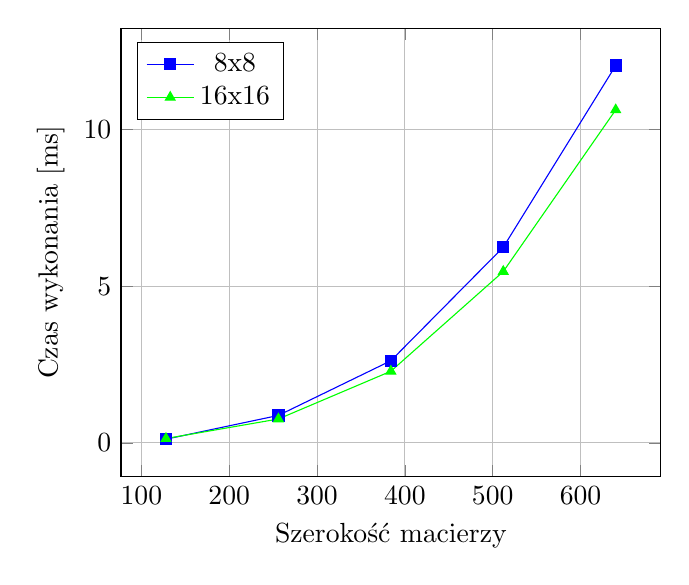
\begin{tikzpicture}
    \begin{axis}[
      xlabel=Szerokość macierzy,
      ylabel={Czas wykonania [ms]},
      legend pos=north west,
      grid=both
    ]

    \addplot[color=blue,mark=square*] coordinates {%
      (128, 0.118)
      (256, 0.877)
      (384, 2.622)
      (512, 6.248)
      (640, 12.047)
    };
    \addlegendentry{8x8}

    \addplot[color=green,mark=triangle*] coordinates {%
      (128, 0.139)
      (256, 0.763)
      (384, 2.287)
      (512, 5.471)
      (640, 10.632)
    };
    \addlegendentry{16x16}

    \end{axis}%
  \end{tikzpicture}%
  }

  \end{minipage}

  \captionsetup{labelformat=andtable}
  \caption{Zależność pomiędzy czasem obliczeń a rozmiarem macierzy -- wersja 5.}
\end{figure}

\paragraph{Ilość operacji zmiennoprzecinkowych na sekundę}

\begin{figure}[H]

  \begin{minipage}[c]{0.46\textwidth}
  \centering
  \resizebox{\textwidth}{!}{%
  \begin{tabular}{|c|c|c|}
  \hline
  \multirow{2}{*}{Rozmiar macierzy} & \multicolumn{2}{c|}{Rozmiar bloku} \\ \cline{2-3}
  & 8x8 & 16x16 \\ \hline
  128x128 & 35.396 & 30.229 \\ \hline
  256x256 & 38.248 & 43.995 \\ \hline
  384x384 & 43.189 & 49.512 \\ \hline
  512x512 & 42.966 & 49.063 \\ \hline
  640x640 & 43.520 & 49.314 \\ \hline
  \end{tabular}
  \captionlistentry[table]{Ilosc operacji zmiennoprzecinkowych na sekundę (GFLOPS) -- wersja 5.}
  }

  \end{minipage}
  \qquad
  \begin{minipage}[c]{0.46\textwidth}
  \centering

  \resizebox{\textwidth}{!}{%
  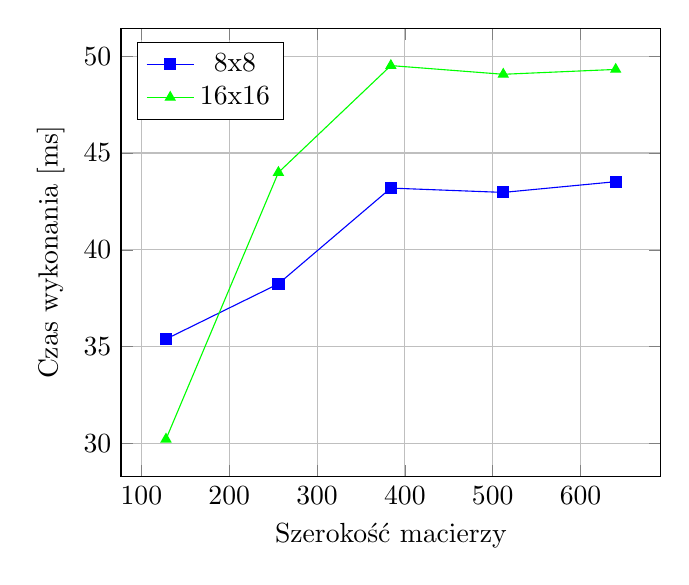
\begin{tikzpicture}
    \begin{axis}[
      xlabel=Szerokość macierzy,
      ylabel={Czas wykonania [ms]},
      legend pos=north west,
      grid=both
    ]

    \addplot[color=blue,mark=square*] coordinates {%
      (128, 35.396)
      (256, 38.248)
      (384, 43.189)
      (512, 42.966)
      (640, 43.520)
    };
    \addlegendentry{8x8}

    \addplot[color=green,mark=triangle*] coordinates {%
      (128, 30.229)
      (256, 43.995)
      (384, 49.512)
      (512, 49.063)
      (640, 49.314)
    };
    \addlegendentry{16x16}

    \end{axis}%
  \end{tikzpicture}%
  }

  \end{minipage}

  \captionsetup{labelformat=andtable}
  \caption{Zależność pomiędzy ilością operacji zmiennoprzecinkowychna sekundę a rozmiarem macierzy -- wersja 5.}
\end{figure}

\paragraph{Ilość instrukcji na sekundę}

\begin{figure}[H]

  \begin{minipage}[c]{0.46\textwidth}
  \centering
  \resizebox{\textwidth}{!}{%
  \begin{tabular}{|c|c|c|c|}
  \hline
  \multirow{2}{*}{Rozmiar macierzy} & \multicolumn{2}{c|}{Rozmiar bloku} \\ \cline{2-3}
  & 8x8 & 16x16 \\ \hline
  128x128 & 0.1481 & 0.1856 \\ \hline
  256x256 & 0.1423 & 0.1641 \\ \hline
  384x384 & 0.1543 & 0.1951 \\ \hline
  512x512 & 0.1574 & 0.1894 \\ \hline
  640x640 & 0.1538 & 0.1909 \\ \hline
  \end{tabular}
  \captionlistentry[table]{Ilość instrukcji wykonana na sekundę (GIPS) -- wersja 5.}
  }

  \end{minipage}
  \qquad
  \begin{minipage}[c]{0.46\textwidth}
  \centering

  \resizebox{\textwidth}{!}{%
  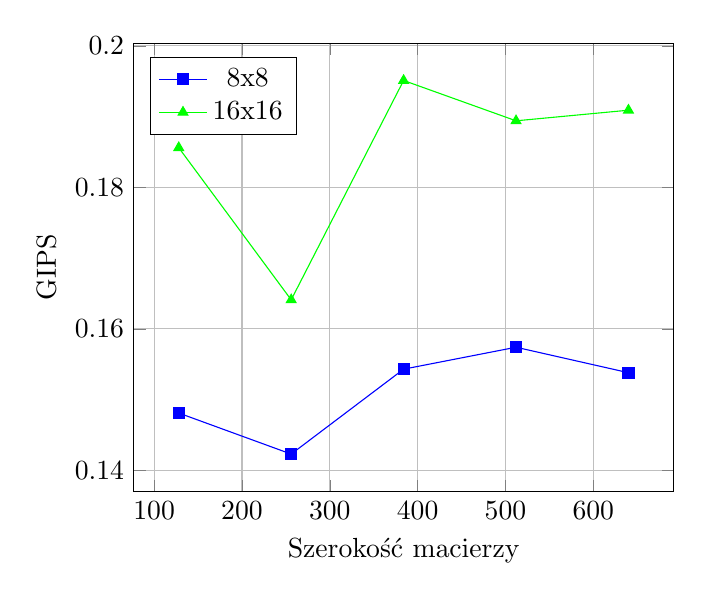
\begin{tikzpicture}
    \begin{axis}[
      xlabel=Szerokość macierzy,
      ylabel={GIPS},
      legend pos=north west,
      grid=both
    ]

    \addplot[color=blue,mark=square*] coordinates {%
      (128, 0.1481)
      (256, 0.1423)
      (384, 0.1543)
      (512, 0.1574)
      (640, 0.1538)
    };
    \addlegendentry{8x8}

    \addplot[color=green,mark=triangle*] coordinates {%
      (128, 0.1856)
      (256, 0.1641)
      (384, 0.1951)
      (512, 0.1894)
      (640, 0.1909)
    };
    \addlegendentry{16x16}

    \end{axis}%
  \end{tikzpicture}%
  }

  \end{minipage}

  \captionsetup{labelformat=andtable}
  \caption{Zależność pomiędzy ilością instrukcji wykonanych na sekundę a rozmiarem macierzy -- wersja 5.}
\end{figure}

\paragraph{CGMA}

\begin{figure}[H]

  \begin{minipage}[c]{0.46\textwidth}
  \centering
  \resizebox{\textwidth}{!}{%
  \begin{tabular}{|c|c|c|c|}
  \hline
  \multirow{2}{*}{Rozmiar macierzy} & \multicolumn{2}{c|}{Rozmiar bloku} \\ \cline{2-3}
  & 8x8 & 16x16 \\ \hline
  128x128 & 240.941 & 1129.931 \\ \hline
  256x256 & 256.250 & 1236.528 \\ \hline
  384x384 & 250.776 & 1276.675 \\ \hline
  512x512 & 253.050 & 1297.743 \\ \hline
  640x640 & 255.393 & 1310.720 \\ \hline
  \end{tabular}
  \captionlistentry[table]{Stosunek ilości operacji zmiennoprzecinkowych do ilości operacji odczytu/zapisu z pamięci globalnej -- wersja 5.}
  }

  \end{minipage}
  \qquad
  \begin{minipage}[c]{0.46\textwidth}
  \centering

  \resizebox{\textwidth}{!}{%
  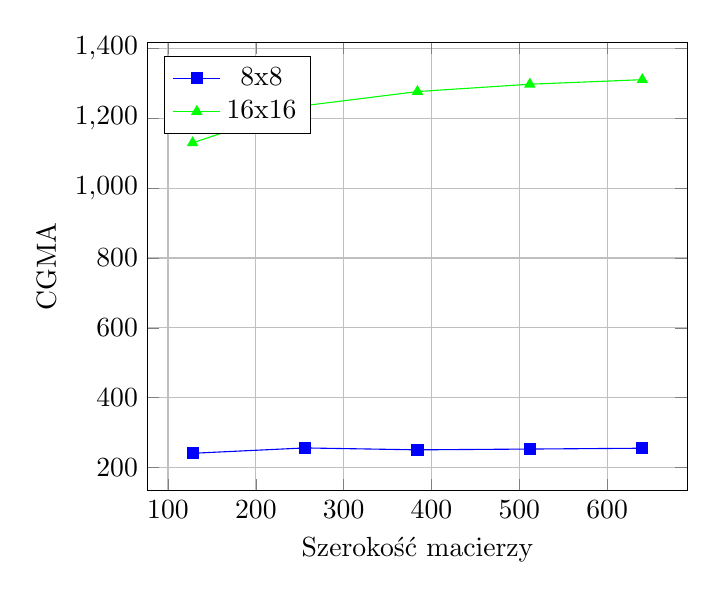
\begin{tikzpicture}
    \begin{axis}[
      xlabel=Szerokość macierzy,
      ylabel={CGMA},
      legend pos=north west,
      grid=both
    ]

    \addplot[color=blue,mark=square*] coordinates {%
      (128, 240.941)
      (256, 256.250)
      (384, 250.776)
      (512, 253.050)
      (640, 255.393)
    };
    \addlegendentry{8x8}

    \addplot[color=green,mark=triangle*] coordinates {%
      (128, 1129.931)
      (256, 1236.528)
      (384, 1276.675)
      (512, 1297.743)
      (640, 1310.720)
    };
    \addlegendentry{16x16}

    \end{axis}%
  \end{tikzpicture}%
  }

  \end{minipage}

  \captionsetup{labelformat=andtable}
  \caption{Zależność CGMA od rozmiaru macierzy -- wersja 4.}
\end{figure}
